\newcommand{\figureBigLCD}[1]{
  \def\lang{\detokenize{#1}}
  \def\langRu{\detokenize{ru}}
  \def\langEn{\detokenize{en}}
  \def\figureCaption{XXX: No translation.}
  \ifx \lang\langRu
  \def\figureCaption{
    Схематическое изображение внешнего вида ЖК-дисплея 20x4 (источник
    изображения:
    \url{https://commons.wikimedia.org/wiki/File:LCD_20x4_breadboard.svg}.)
  }
  \fi
  \ifx \lang\langEn
  \def\figureCaption{
    A schematic representation of the outer appearance of an 20x4 LCD (image
    source:
    \url{https://commons.wikimedia.org/wiki/File:LCD_20x4_breadboard.svg}.)
  }
  \fi
  \begin{figure}[h]
    \centering
    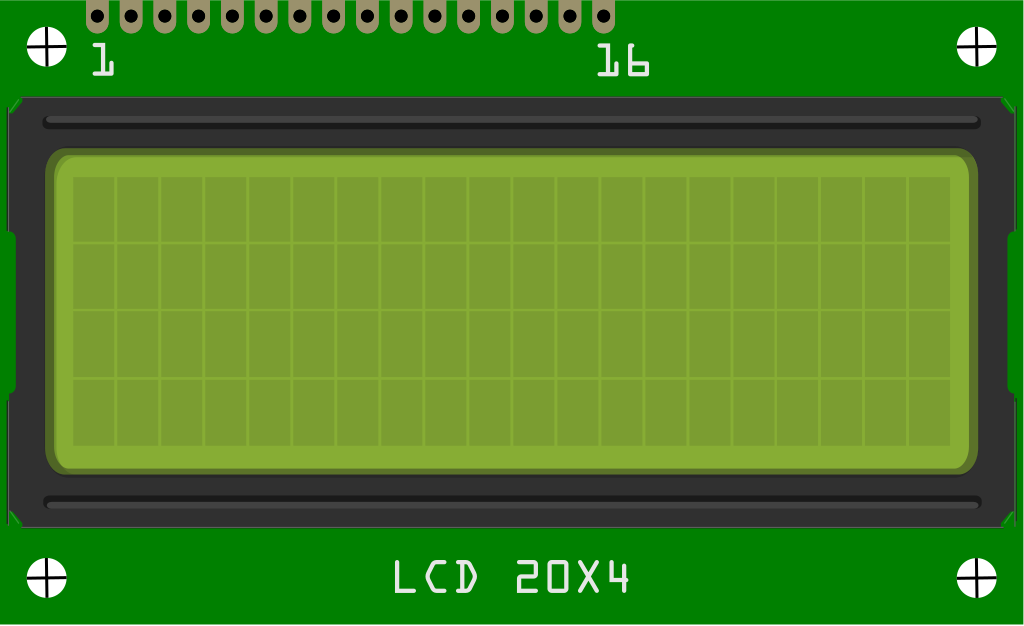
\includegraphics[width=10cm]{lcd-20x4}
    \caption{\figureCaption}
    \label{fig:lcd-20x4}
  \end{figure}
}
